% !TEX program = pdflatex
% !TEX options = -shell-escape
\documentclass[14pt, russian]{scrartcl}
\let\counterwithout\relax
\let\counterwithin\relax
\usepackage{float}
\usepackage{xcolor}
\usepackage{extsizes}
\usepackage{subfig}
\usepackage[export]{adjustbox}
\usepackage{tocvsec2}
\usepackage[subfigure]{tocloft}

\AtBeginEnvironment{figure}{\vspace{0.5cm}}
\AtBeginEnvironment{table}{\vspace{0.5cm}}
\AtBeginEnvironment{listing}{\vspace{0.5cm}}
\AtBeginEnvironment{algorithm}{\vspace{0.5cm}}
\usepackage{ulem,bm,mathrsfs,ifsym}
\normalem
\renewcommand{\emph}[1]{#1}
\usepackage{sectsty}

%%% Поля и разметка страницы %%%
\usepackage{pdflscape}
\usepackage{geometry}
\geometry{a4paper,tmargin=2cm,bmargin=2cm,lmargin=3cm,rmargin=1cm}

%%% Математические пакеты %%%
\usepackage{amsthm,amsfonts,amsmath,amssymb,amscd}
\usepackage{mathtools}
\usepackage[perpage]{footmisc}

\KOMAoptions{fontsize=14pt}

\makeatletter
\def\showfontsize{\f@size{} point}
\makeatother

\makeatletter
\setlength{\@fptop}{0pt}
\makeatother

\usepackage{tempora}
\usepackage{cmap}
\usepackage[T2A,T1]{fontenc}
\usepackage[utf8]{inputenc}
\usepackage[english, main=russian]{babel}
\usepackage{textcomp}
\usepackage{indentfirst}

%%% Таблицы %%%
\usepackage{longtable}
\usepackage{multirow,makecell,array}
\usepackage{booktabs}

%%% Общее форматирование
\usepackage{soulutf8}
\usepackage{icomma}

%%% Изображения %%%
\usepackage{graphicx}
\usepackage{wrapfig}

%%% Списки %%%
\usepackage{enumitem}

%%% Подписи %%%
\usepackage{caption}

\addto\captionsrussian{%
  \renewcommand{\lstlistingname}{Листинг}%
}
%%% Счётчики %%%
\usepackage[figure,table,section]{totalcount}
\DeclareTotalCounter{lstlisting}
\usepackage{totcount}
\usepackage{totpages}

\linespread{1.3}

%%% Гиперссылки %%%
\usepackage{hyperref}

%%% Выравнивание и переносы %%%
\sloppy
\clubpenalty=10000
\widowpenalty=10000

\makeatletter
\let\@@scshape=\scshape
\renewcommand{\scshape}{%
  \ifnum\strcmp{\f@series}{bx}=\z@
    \usefont{T1}{cmr}{bx}{sc}%
  \else
    \ifnum\strcmp{\f@shape}{it}=\z@
      \fontshape{scsl}\selectfont
    \else
      \@@scshape
    \fi
  \fi}
\makeatother

\usepackage{ifthen}
\newcounter{intvl}
\newcounter{otstup}
\newcounter{contnumeq}
\newcounter{contnumfig}
\newcounter{contnumtab}
\newcounter{pgnum}
\newcounter{bibliosel}
\newcounter{chapstyle}
\newcounter{headingdelim}
\newcounter{headingalign}
\newcounter{headingsize}
\newcounter{tabcap}
\newcounter{tablaba}
\newcounter{tabtita}

\setcounter{intvl}{3}
\setcounter{otstup}{0}
\setcounter{contnumeq}{1}
\setcounter{contnumfig}{1}
\setcounter{contnumtab}{1}
\setcounter{pgnum}{0}
\setcounter{bibliosel}{1}
\setcounter{chapstyle}{1}
\setcounter{headingdelim}{1}
\setcounter{headingalign}{0}
\setcounter{headingsize}{0}
\setcounter{tabcap}{0}
\setcounter{tablaba}{2}
\setcounter{tabtita}{1}

\DeclareCaptionLabelSeparator*{emdash}{~--- }
\captionsetup[listing]{position=top,labelsep=colon,justification=centering,singlelinecheck=false}
\captionsetup[lstlisting]{position=top,labelsep=colon,justification=centering,singlelinecheck=false}
\captionsetup[figure]{labelsep=emdash,font=onehalfspacing,position=bottom}

\ifthenelse{\equal{\thetabcap}{0}}{%
    \newcommand{\tabcapalign}{\raggedright}
}

\DeclareCaptionFormat{tablecaption}{\tabcapalign #1#2#3}
\captionsetup[table]{labelsep=emdash}
\captionsetup[table]{format=tablecaption,singlelinecheck=off,font=onehalfspacing,position=top,skip=-5pt}
\DeclareCaptionLabelFormat{continued}{Продолжение таблицы~#2}
\setlength{\belowcaptionskip}{.2cm}
\setlength{\intextsep}{0ex}

\renewcommand{\thesubfigure}{\asbuk{subfigure}}
\captionsetup[subfigure]{font={normalsize},
    labelformat=brace,
    justification=centering,
}

\definecolor{linkcolor}{rgb}{0.0,0,0}
\definecolor{citecolor}{rgb}{0,0.0,0}
\definecolor{urlcolor}{rgb}{0,0,0}

\hypersetup{
    linktocpage=true,
    plainpages=true,
    unicode=true,
    colorlinks,
    linkcolor={linkcolor},
    citecolor={citecolor},
    urlcolor={urlcolor},
    pdflang={ru},
}
\urlstyle{same}

\setlength{\parindent}{2.5em}

\renewcommand{\labelitemi}{---}
\setlist{nosep,
    labelindent=\parindent,leftmargin=*
}

\usepackage{ragged2e}
\usepackage{needspace}
\usepackage[explicit]{titlesec}
\usepackage{placeins}
\usepackage{xparse}
\usepackage{csquotes}

\usepackage[highlightmode=immediate]{minted}
\usepackage{listings}
\providecommand{\listingname}{Листинг}
\addto\captionsrussian{%
  \renewcommand{\listingname}{Листинг}%
}
\lstset{
  basicstyle=\ttfamily\footnotesize,
  breakatwhitespace=false,
  breaklines=true,
  captionpos=t,
  inputencoding=utf8,
  frame=single,
  keepspaces=true,
  keywordstyle=\bf,
  numbers=left,
  numbersep=5pt,
  xleftmargin=25pt,
  xrightmargin=25pt,
  showspaces=false,
  showstringspaces=false,
  showtabs=false,
  stepnumber=1,
  tabsize=2,
  title=\lstname
}
\setminted{
  frame=single,
  fontsize=\footnotesize,
  linenos,
  xleftmargin=1.5em,
  breaklines=true,
}
\newenvironment{longlisting}{\captionsetup{type=listing}}{}
\usepackage{url}
\usepackage{algorithm, algorithmicx}
\usepackage[noend]{algpseudocode}
\usepackage{blkarray}
\usepackage{chngcntr}
\usepackage{tabularx}
\usepackage{tikz}
\usetikzlibrary{shapes.geometric, arrows.meta, positioning}

% --- Библиография ---
\usepackage[backend=biber,
    bibstyle=gost-numeric,
    citestyle=nature]{biblatex}
\addbibresource{biblio.bib}
% Как в РПЗ: [Электронный ресурс] у @online (поле media = {eresource} в .bib)
\DefineBibliographyStrings{russian}{%
  mediaeresource = {{Электронный ресурс}},%
}

\titleformat{name=\section,numberless}[block]{\normalfont\Large\centering}{}{0em}{#1}
\titleformat{\section}[block]{\normalfont\Large\bfseries\raggedright}{}{0em}{\thesection\hspace{0.25em}#1}
\titleformat{\subsection}[block]{\normalfont\Large\bfseries\raggedright}{}{0em}{\thesubsection\hspace{0.25em}#1}
\titleformat{\subsubsection}[block]{\normalfont\large\bfseries\raggedright}{}{0em}{\thesubsubsection\hspace{0.25em}#1}

\let\Algorithm\algorithm
\renewcommand\algorithm[1][]{\Algorithm[#1]\setstretch{1.5}}

\usepackage{pifont}
\usepackage{calc}
\usepackage{suffix}
\DeclareQuoteStyle{russian}
    {\guillemotleft}{\guillemotright}[0.025em]
    {\quotedblbase}{\textquotedblleft}
\ExecuteQuoteOptions{style=russian}
\newcommand{\enq}[1]{\enquote{#1}}
\newcommand{\eng}[1]{\begin{english}#1\end{english}}

\definecolor{mygreen}{rgb}{0,0.6,0}
\definecolor{mygray}{rgb}{0.5,0.5,0.5}
\definecolor{mymauve}{rgb}{0.58,0,0.82}
\renewcommand{\listalgorithmname}{Список алгоритмов}
\floatname{algorithm}{Листинг}
\renewcommand{\lstlistingname}{Листинг}
\renewcommand{\thealgorithm}{\arabic{algorithm}}

\newcommand{\refAlgo}[1]{(листинг \ref{#1})}
\newcommand{\refImage}[1]{(рисунок \ref{#1})}

\renewcommand{\theenumi}{\arabic{enumi}.}
\renewcommand{\labelenumi}{\arabic{enumi}.}
\renewcommand{\theenumii}{\arabic{enumii}}
\renewcommand{\labelenumii}{(\arabic{enumii})}
\renewcommand{\theenumiii}{\roman{enumiii}}
\renewcommand{\labelenumiii}{(\roman{enumiii})}
\renewcommand{\labelitemi}{---}
\renewcommand{\labelitemii}{---}

\lstdefinelanguage{Refal}{
  sensitive=true,
  morecomment=[s]{/*}{*/},
  commentstyle=\color{mygreen},
  morestring=[b]',
  stringstyle=\color{mymauve}
}

\makeatletter
\def\p@subsection{}
\def\p@subsubsection{\thesection\,\thesubsection\,}
\makeatother
\newcommand{\prog}[1]{{\ttfamily\small#1}}

\newcommand{\anonsection}[1]{\cleardoublepage
\phantomsection
\addcontentsline{toc}{section}{\protect\numberline{}#1}
\section*{#1}\vspace*{2.5ex}}
\newcommand{\sectionbreak}{\clearpage}
\renewcommand{\sectionfont}{\normalsize}
\renewcommand{\cftsecleader}{\cftdotfill{\cftdotsep}}

\renewcommand{\cftsecfont}{\normalfont\large}
\renewcommand{\cftsubsecfont}{\normalfont\large}

\setlength{\cftsecindent}{0pt}
\setlength{\cftsubsecindent}{0pt}
\setlength{\cftsubsubsecindent}{0pt}

\usepackage{caption}
\usepackage{amsmath}
\usepackage{amsfonts}
\usepackage{mathtools}
    \DeclarePairedDelimiter\abs{\lvert}{\rvert}
    \DeclarePairedDelimiter\norm{\lVert}{\rVert}
\DeclareTextCommandDefault{\textvisiblespace}{%
  \mbox{\kern.06em\vrule \@height.3ex}%
  \vbox{\hrule \@width.3em}%
  \hbox{\vrule \@height.3ex}}
\newsavebox{\spacebox}
\begin{lrbox}{\spacebox}
\verb*! !
\end{lrbox}
\newcommand{\aspace}{\usebox{\spacebox}}
\DeclareTotalCounter{listing}

\makeatletter
\renewcommand*{\p@subsubsection}{}
\makeatother

\begin{document}
\sloppy

\def\figurename{Рисунок}

\begin{titlepage}
\thispagestyle{empty}
\newpage

\vspace*{-30pt}
\hspace{-45pt}
\begin{minipage}{0.17\textwidth}
\hspace*{-20pt}\centering

\includegraphics[width=1.3\textwidth]{../nir/Emblem.png}
\end{minipage}
\begin{minipage}{0.82\textwidth}\small \textbf{
\vspace*{-0.7ex}
\hspace*{-10pt}\centerline{Министерство науки и высшего образования Российской Федерации}
\vspace*{-0.7ex}
\centerline{Федеральное государственное автономное образовательное учреждение }
\vspace*{-0.7ex}
\centerline{высшего образования}
\vspace*{-0.7ex}
\centerline{<<Московский государственный технический университет}
\vspace*{-0.7ex}
\centerline{имени Н.Э. Баумана}
\vspace*{-0.7ex}
\centerline{(национальный исследовательский университет)>>}
\vspace*{-0.7ex}
\centerline{(МГТУ им. Н.Э. Баумана)}}
\end{minipage}

\vspace{-2pt}
\hspace{-34.5pt}\rule{\textwidth}{2.5pt}

\vspace*{-20.3pt}
\hspace{-34.5pt}\rule{\textwidth}{0.4pt}

\vspace{0.5ex}
\noindent \small ФАКУЛЬТЕТ\hspace{80pt} <<Информатика и системы управления>>

\vspace*{-16pt}
\hspace{35pt}\rule{0.855\textwidth}{0.4pt}

\vspace{0.5ex}
\noindent \small КАФЕДРА\hspace{50pt} <<Теоретическая информатика и компьютерные технологии>>

\vspace*{-16pt}
\hspace{25pt}\rule{0.875\textwidth}{0.4pt}

\vspace{3em}

\begin{center}
\Large \bf{РАСЧЕТНО-ПОЯСНИТЕЛЬНАЯ ЗАПИСКА\\\textbf{\textit{К ПРЕДДИПЛОМНОЙ ПРАКТИКЕ\\НА ТЕМУ:}} \\}
\end{center}

\vspace*{-6ex}
\begin{center}
\Large
\textit{\textbf{«\,Компилятор базисного подмножества}}\par
\vspace*{-3ex}
\rule{0.9\textwidth}{1.2pt}

\vspace*{0.55ex}
\textit{\textbf{Рефала-5 с представлением данных,}}\par
\vspace*{-3ex}
\rule{0.9\textwidth}{1.2pt}

\vspace*{0.55ex}
\textit{\textbf{использующим раскрученные очереди\,»}}\par
\vspace*{-3ex}
\rule{0.9\textwidth}{1.2pt}

\vspace*{-0.2ex}
\rule{0.9\textwidth}{1.2pt}

\vspace*{-0.2ex}
\rule{0.9\textwidth}{1.2pt}
\end{center}

\vspace{\fill}

\newlength{\ML}
\settowidth{\ML}{«\underline{\hspace{0.7cm}}» \underline{\hspace{2cm}}}

\noindent Студент \underline{\hspace{1.5cm}} \hfill \underline{\hspace{4cm}}\quad
\underline{\hspace{4cm}}

\vspace{-2.1ex}
\noindent\hspace{9ex}\scriptsize{(Группа)}\normalsize\hspace{170pt}\hspace{2ex}\scriptsize{(Подпись, дата)}\normalsize\hspace{30pt}\hspace{6ex}\scriptsize{(И.О. Фамилия)}\normalsize

\bigskip

\noindent Руководитель  \hfill \underline{\hspace{4cm}}\quad
\underline{\hspace{4cm}}

\vspace{-2ex}
\noindent\hspace{13.5ex}\normalsize\hspace{170pt}\hspace{2ex}\scriptsize{(Подпись, дата)}\normalsize\hspace{30pt}\hspace{6ex}\scriptsize{(И.О. Фамилия)}\normalsize
\vfill

\begin{center}
\textsl{\the\year{} г.}
\end{center}
\end{titlepage}

\setlength{\tabcolsep}{3pt}
\newpage
\setcounter{page}{2}

\renewcommand\contentsname{\hfill{\normalfont{СОДЕРЖАНИЕ}}\hfill}
\tableofcontents
\newpage

\anonsection{ВВЕДЕНИЕ}

Рефал-5~--- язык программирования, в основе которого лежит переписывание
объектных выражений по набору правил. Программа на Рефале задаётся как
функции, состоящие из предложений вида «образец $\to$ результат»;
интерпретатор сопоставляет аргументы вызова с образцами и собирает
правую часть подошедшего предложения. Скорость такой машины определяется
не только тем, сколько шагов нормализации она делает, но и тем, как
устроены сами операции над объектными выражениями: вставка с концов,
извлечение, конкатенация.

Цель производственной практики~--- довести до работающего состояния
реализацию базисного подмножества Рефала-5 на Java, в которой объектное
выражение представлено раскрученной (bootstrapped) двусторонней очередью
по Окасаки. От этой структуры ожидается амортизированно константная
конкатенация, и на её фоне реализация должна обогнать классические
списочные интерпретаторы Рефала-5 на программах, где такая конкатенация
встречается на каждом шаге нормализации.

Конкретные задачи, поставленные на практику:
\begin{itemize}
  \item реализовать структуру данных \prog{Expr} (мелкий и глубокий
        уровни, конкатенация по четырём случаям) и итеративный цикл
        нормализации с двумя стеками;
  \item написать тестовый каркас, в который входят юнит-тесты, интеграционные
        проверки и прогон чужих наборов автотестов;
  \item оформить инструкцию пользователя: сборка, запуск, опции командной
        строки, коды возврата;
  \item провести сравнительный замер с Refal-5~PZ и Refal-5J на программе,
        где списочное представление даёт квадратичную сложность,
        и подтвердить или опровергнуть теоретическое преимущество.
\end{itemize}

Теоретическое обоснование выбора структуры данных (мелкий и глубокий
уровни, инварианты, ребалансировка, амортизированные оценки) сделано
в рамках научно-исследовательской работы и в отчёте по практике не
повторяется. Здесь акцент смещён на инженерную сторону: что именно
реализовано, как оно тестируется и какие числа даёт на стенде.

\section{Технологическая часть}
\label{sec:tech}

\subsection{Инструкция пользователя}
\label{subsec:user-manual}

\subsubsection{Требования к среде}

Для сборки и запуска интерпретатора необходимо следующее программное обеспечение
(таблица~\ref{tab:requirements}). Проверка наличия и версий выполняется
командами \prog{java -\/\/-version}, \prog{mvn -\/\/-version} в терминале.

\begin{table}[!htb]
\caption{\centering Требования к среде разработки}
\label{tab:requirements}
\centering
\small
\begin{tabular}{@{}lll@{}}
\toprule
\textbf{Компонент} & \textbf{Минимальная версия} & \textbf{Примечание} \\
\midrule
Java Development Kit & 25 LTS & Сборка и запуск \\
Apache Maven & 3.9.x & Сборка проекта \\
Python~3 & 3.9+ & Только для построения графиков \\
\bottomrule
\end{tabular}
\end{table}

\subsubsection{Сборка}

Проект собирается командой Apache~Maven из корня репозитория \prog{refal5j-impl/}:

\begin{longlisting}
\caption{Команда сборки}\label{lst:build}
\begin{minted}{bash}
mvn package -DskipTests
\end{minted}
\end{longlisting}

Результат сборки --- файл \prog{target/refal5q.jar}, самодостаточный
JAR-архив с прописанным классом \prog{Main-Class: refal.Main}.
Все зависимости рантайма включены в него через плагин Maven~Shade,
поэтому для запуска достаточно стандартной JVM без дополнительных библиотек.

Сборка с полным прогоном тестов выполняется командой \prog{mvn package}
(без флага \prog{-DskipTests}) или \prog{mvn verify}, которая дополнительно
формирует отчёт о покрытии кода инструментом JaCoCo.

\newpage
\subsubsection{Запуск интерпретатора}

Интерпретатор запускается через стандартную команду \prog{java -jar}:

\begin{longlisting}
\caption{Форма запуска}\label{lst:run}
\begin{minted}{bash}
java -jar target/refal5q.jar [OPTIONS] program.ref
\end{minted}
\end{longlisting}

Позиционный аргумент --- путь к исходному файлу \prog{.ref}.
Поддерживаемые опции перечислены в таблице~\ref{tab:options}.

\begin{table}[!htb]
\caption{\centering Опции командной строки}
\label{tab:options}
\centering
\small
\begin{tabular}{@{}lp{8.5cm}@{}}
\toprule
\textbf{Опция} & \textbf{Описание} \\
\midrule
\prog{--entry <имя>} &
    Явное указание входной функции; имеет приоритет над \prog{\$ENTRY} в файле \\
\prog{--step-limit <N>} &
    Максимальное число шагов нормализации (по умолчанию~--- 100\,000) \\
\prog{--expr <терм...>} &
    Начальное выражение, передаваемое входной функции вместо пустого \\
\bottomrule
\end{tabular}
\end{table}

Код завершения процесса отражает результат выполнения
(таблица~\ref{tab:exit-codes}).

\begin{table}[!htb]
\caption{\centering Коды завершения процесса}
\label{tab:exit-codes}
\centering
\small
\begin{tabular}{@{}cl@{}}
\toprule
\textbf{Код} & \textbf{Условие} \\
\midrule
0 & Успешное завершение или \prog{<Exit 0>} \\
1 & Ошибка лексического, синтаксического или семантического анализа \\
2 & Ошибка времени выполнения: нет подходящего правила,
    превышение лимита шагов \\
$n$ & Значение $n$, переданное встроенной функции \prog{<Exit~n>} \\
\bottomrule
\end{tabular}
\end{table}

Пример запуска программы \prog{hello.ref} с явным указанием точки входа:

\begin{longlisting}
\caption{Пример запуска}\label{lst:run-example}
\begin{minted}{bash}
java -jar target/refal5q.jar --entry Go hello.ref
\end{minted}
\end{longlisting}

\subsubsection{Запуск тестов}

Полный набор тестов запускается одной командой Maven:

\newpage
\begin{longlisting}
\caption{Запуск тестов}\label{lst:test}
\begin{minted}{bash}
mvn test
mvn verify
mvn test -Dtest=AutotestsRunnerTest
\end{minted}
\end{longlisting}

Первые две команды прогоняют 143~JUnit-теста, покрывающих все компоненты
проекта. Третья команда запускает отдельный класс \prog{AutotestsRunnerTest},
который вызывает интерпретатор на 81~внешней программе из двух наборов:
автотесты репозитория \prog{refal-5j} и десахаренные тесты репозитория
\prog{refal-5-framework}. Каждая программа выполняется в отдельном процессе
с тайм-аутом 20~секунд.

Отчёт JaCoCo формируется в каталоге \prog{target/site/jacoco/}; открыть
его можно браузером, указав путь к \prog{index.html}.

%%% ─────────────────────────────────────────────────────────
\subsection{Структура данных: раскрученная двусторонняя очередь}
\label{subsec:deque-impl}

Объектное выражение в нашей реализации хранится в раскрученной (bootstrapped)
двусторонней очереди по Окасаки~\cite{okasaki_pfds}. У неё амортизированно
константная конкатенация~--- та самая операция, на которой классические
списочные интерпретаторы Рефала (включая Refal-5~PZ и Refal-5J) тратят
линейное время.

\subsubsection{Sealed interface Expr<T>}

Контейнер выражения объявлен как обобщённый запечатанный интерфейс с двумя
реализациями:

\begin{longlisting}
\caption{Запечатанный интерфейс Expr<T>}\label{lst:expr-iface}
\begin{minted}{java}
public sealed interface Expr<T> extends Iterable<T>
        permits ShallowDeque, DeepDeque {
    boolean isEmpty();
    int size();
    PeekResult<T> separateFront();
    PeekResult<T> separateBack();
    Expr<T> pushFront(T x);
    Expr<T> pushBack(T x);
    static <T> Expr<T> empty()        { return ShallowDeque.empty(); }
    static <T> Expr<T> singleton(T x) { return ShallowDeque.<T>empty().pushBack(x); }
    static <T> Expr<T> concat(Expr<T> a, Expr<T> b) { return ExprOps.concat(a, b); }
}
\end{minted}
\end{longlisting}

Слово \prog{sealed} запрещает любые другие наследники. Компилятор
Java~25 на этом основании проверяет полноту разбора в
\prog{switch}-выражениях, поэтому в коде конкатенации мы можем
перечислить ровно четыре случая по типам операндов и не писать ветку
\prog{default}: её отсутствие гарантировано системой типов.

\subsubsection{Параметры буферов}

Ёмкость мелкого буфера~--- константа \prog{ShallowDeque.CAPACITY = 9},
нижняя граница заполненности \prog{MIN\_FILL = 5}, то есть
$\lceil CAPACITY / 2 \rceil$. Нечётное значение выбрано по
арифметическим соображениям: при переполнении мелкого буфера суммарно
получается $CAPACITY + 1 = 10$ элементов; они делятся ровно пополам
на два фрагмента по 5, и оба фрагмента сразу удовлетворяют
\prog{MIN\_FILL}. С чётной ёмкостью пришлось бы либо мириться с
остатком в один элемент, либо добавлять отдельную обработку этого
случая~--- ни то ни другое не даёт выигрыша по свойствам структуры.

На практике глубина рекурсии \prog{DeepDeque} при таком \prog{CAPACITY}
почти не выходит за два уровня: в тестовых программах с выражениями
длиной до десятков тысяч термов средняя очередь сама ни разу не успевает
стать глубокой.

\subsubsection{ShallowDeque<T>: мелкий буфер}

\prog{ShallowDeque<T>}~--- иммутабельный класс с тремя полями:
массив фиксированной длины \prog{Object[] buf} размером \prog{CAPACITY},
индекс головы \prog{head} и текущий размер \prog{sz}.
Доступ по логическому индексу~$i$ выполняется через единственную формулу:

\newpage
\begin{longlisting}
\caption{Циклическое индексирование в ShallowDeque}\label{lst:shallow-idx}
\begin{minted}{java}
int idx(int i) {
    return Math.floorMod(head + i, CAPACITY);
}
\end{minted}
\end{longlisting}

\prog{floorMod} здесь стоит вместо обычного \prog{\%}, потому что в Java
оператор \prog{\%} при отрицательном делимом возвращает отрицательный
остаток, а нам нужен индекс в массиве. \prog{pushFrontTight} как раз
сдвигает голову на~$-1$, и без \prog{floorMod} в этой точке пришлось бы
вручную добавлять \prog{CAPACITY}.

В классе определены два варианта операций добавления:
\begin{itemize}
  \item \prog{pushFrontTight(T)} и \prog{pushBackTight(T)}~--- внутренние, возвращают
        \prog{ShallowDeque<T>} и бросают \prog{IllegalStateException} при переполнении;
        применяются там, где вызывающий код гарантирует наличие свободного места
        (например, при формировании буферов во время конкатенации);
  \item \prog{pushFront(T)} и \prog{pushBack(T)}~--- публичные (методы
        интерфейса \prog{Expr<T>}); при переполнении автоматически переходят
        в глубокий уровень через \prog{DeepDeque.mkDeep}.
\end{itemize}

\subsubsection{DeepDeque<T>: глубокий уровень}

\prog{DeepDeque<T>} реализует тройку $\langle front, mid, back \rangle$:

\begin{longlisting}
\caption{Поля DeepDeque<T>}\label{lst:deep-fields}
\begin{minted}{java}
public final class DeepDeque<T> implements Expr<T> {
    private final ShallowDeque<T>          front;
    private final Expr<ShallowDeque<T>>    mid;
    private final ShallowDeque<T>          back;
    private final int                      sz;
    ...
}
\end{minted}
\end{longlisting}

Тип поля \prog{mid}~--- \prog{Expr<ShallowDeque<T>>}, и именно здесь
проявляется «раскрутка»: средняя очередь хранит мелкие буферы, но сама
она тоже \prog{Expr<\ldots>}, то есть может оказаться как
\prog{ShallowDeque}, так и \prog{DeepDeque} следующего уровня.
На разумных размерах выражений рекурсия редко уходит глубже второго
уровня.

Конструктор \prog{mkDeep} автоматически схлопывает глубокую очередь обратно
в мелкую, когда суммарное число элементов не превышает \prog{CAPACITY}:

\begin{longlisting}
\caption{Конструктор mkDeep с откатом в ShallowDeque}\label{lst:mkdeep}
\begin{minted}{java}
static <T> Expr<T> mkDeep(ShallowDeque<T> front,
                           Expr<ShallowDeque<T>> mid,
                           ShallowDeque<T> back, int total) {
    if (total <= CAPACITY) {
        ShallowDeque<T> flat = ShallowDeque.empty();
        for (T x : iterableOf(front))  flat = flat.pushBackTight(x);
        for (ShallowDeque<T> bucket : iterableOf(mid))
            for (T x : iterableOf(bucket)) flat = flat.pushBackTight(x);
        for (T x : iterableOf(back))   flat = flat.pushBackTight(x);
        return flat;
    }
    return new DeepDeque<>(front, mid, back, total);
}
\end{minted}
\end{longlisting}

Параметр \prog{total} передаётся явно, чтобы не пересчитывать его внутри:
\prog{mid.size()} возвращает число буферов в средней очереди, а не суммарное
число листовых элементов, поэтому наивная формула
\prog{front.size() + mid.size() + back.size()} оказалась бы некорректной.
Каждый вызов \prog{mkDeep} обновляет \prog{total} инкрементально~---
прибавляя или вычитая единицу по ходу операции добавления или извлечения.

\subsubsection{Конкатенация: четыре случая}

Конкатенация реализована в служебном классе \prog{ExprOps} с разбором
четырёх случаев по мелкости/глубине операндов:

\begin{longlisting}
\caption{Разбор четырёх случаев конкатенации}\label{lst:concat-cases}
\begin{minted}{java}
static <T> Expr<T> concat(Expr<T> a, Expr<T> b) {
    if (a.isEmpty()) return b;
    if (b.isEmpty()) return a;
    if (a instanceof ShallowDeque<T> sa && b instanceof ShallowDeque<T> sb)
        return concatSS(sa, sb);
    if (a instanceof ShallowDeque<T> sa && b instanceof DeepDeque<T> db)
        return concatSD(sa, db);
    if (a instanceof DeepDeque<T> da && b instanceof ShallowDeque<T> sb)
        return concatDS(da, sb);
    DeepDeque<T> da = (DeepDeque<T>) a;
    DeepDeque<T> db = (DeepDeque<T>) b;
    return concatDD(da, db);
}
\end{minted}
\end{longlisting}

В случае \emph{Deep\,+\,Deep} пограничные буферы \prog{a.back} и
\prog{b.front} склеиваются в один буфер, а \prog{concat} вызывается
рекурсивно уже на средних очередях. На каждом уровне рекурсии работа
ограничена константой, а сама рекурсия идёт не глубже логарифма от
длины выражения~--- так Окасаки и получает амортизированную
константу~\cite{okasaki_pfds}.

%%% ─────────────────────────────────────────────────────────
\subsection{Цикл нормализации}
\label{subsec:runtime-impl}

\subsubsection{Поле зрения и иерархия ViewTerm}

Нормализация выражения выполняется итеративным проходом по
\emph{полю зрения}~--- линейной последовательности элементарных единиц.
Каждая такая единица описывается запечатанным интерфейсом \prog{ViewTerm}:

\begin{longlisting}
\caption{Иерархия ViewTerm}\label{lst:viewterm}
\begin{minted}{java}
public sealed interface ViewTerm
        permits ViewTerm.Passive,  ViewTerm.BulkPassive,
                ViewTerm.AngOpen,  ViewTerm.AngClose,
                ViewTerm.ParenOpen, ViewTerm.ParenClose {

    record Passive(Term term)          implements ViewTerm {}
    record BulkPassive(Expr<Term> items) implements ViewTerm {}
    record AngOpen(String fn)          implements ViewTerm {}
    record AngClose()                  implements ViewTerm {}
    record ParenOpen()                 implements ViewTerm {}
    record ParenClose()                implements ViewTerm {}
}
\end{minted}
\end{longlisting}

Термы-атомы (\prog{Sym}, \prog{Num}, \prog{Str}) и скобочные термы \prog{Br}
после нормализации вложенных выражений представляются как \prog{Passive}.
Вызов \prog{<f args>} разворачивается в последовательность
\prog{AngOpen(f)}, элементы аргументов, \prog{AngClose}.
Скобочный терм~\prog{(e.X)} аналогично разворачивается через
\prog{ParenOpen} и \prog{ParenClose}.
\prog{BulkPassive} отвечает за оптимизацию связывания переменных и описан
в следующем подразделе.

\subsubsection{Двустековая реализация нормализатора}

Нормализация работает с двумя стеками~--- \prog{left} и \prog{right}:
\begin{itemize}
  \item \prog{right} содержит ещё не обработанные элементы поля зрения;
  \item \prog{left} накапливает уже пассивные элементы~--- те, в которых
        не осталось ни одного активного вызова.
\end{itemize}

Исходное выражение сначала сплющивается в \prog{right} слева-направо.
Затем главный цикл извлекает элементы из \prog{right} по одному с головы.
Пассивные элементы (\prog{Passive}, \prog{BulkPassive}) и открывающие
маркеры (\prog{AngOpen}, \prog{ParenOpen}) просто перекладываются в
\prog{left}. Обработка наступает при встрече закрывающего маркера:

\begin{longlisting}
\caption{Обработка закрывающего маркера вызова функции}\label{lst:angclose}
\begin{minted}{java}
case ViewTerm.AngClose ignored -> {
    bumpStep();
    Expr<Term> argsExpr = Expr.empty();
    String fn = null;
    while (true) {
        ViewTerm top = left.pollLast();
        if (top instanceof ViewTerm.AngOpen ao) { fn = ao.fn(); break; }
        if (top instanceof ViewTerm.Passive pt)
            argsExpr = argsExpr.pushFront(pt.term());
        else if (top instanceof ViewTerm.BulkPassive bp)
            argsExpr = Expr.concat(bp.items(), argsExpr); // O(1)
    }
}
\end{minted}
\end{longlisting}

При встрече \prog{AngClose} мы снимаем элементы с хвоста \prog{left}
до парного \prog{AngOpen} и попутно собираем выражение аргументов
\prog{argsExpr}. Одиночный \prog{Passive} присоединяется через
\prog{pushFront} за~$O(1)$, а \prog{BulkPassive}~--- через
\prog{Expr.concat(bp.items(), argsExpr)}, тоже за~$O(1)$
амортизированно. Обработка \prog{ParenClose} устроена точно так же,
только без поиска имени функции.

После сборки аргументов для встроенной функции результат сплющивается и
помещается обратно в \prog{right}; для пользовательской функции находится
первое подходящее правило и его правая часть, с подставленными связываниями
переменных, укладывается на \prog{right} методом
\prog{pushResultToStack}.

Итеративный цикл вместо рекурсивного обхода даёт нам независимость от
размера стека JVM: сколь угодно глубоко вложенная рефал-программа
обрабатывается в константной глубине Java-стека, а реальный расход
памяти зависит только от длины поля зрения.

\subsubsection{Оптимизация BulkPassive}
\label{subsubsec:bulkpassive}

Без оптимизации подстановка значения переменной в правой части правила
требовала поэлементной укладки: каждый \prog{Term} из связанного значения
помещался на стек \prog{right} как отдельный объект \prog{Passive}:

\begin{longlisting}
\caption{Наивная укладка переменной (до оптимизации)}\label{lst:var-naive}
\begin{minted}{java}
case refal.ast.Var v -> {
    Expr<Term> val = bindings.get(v.key());
    // O(N) итераций: каждый терм становится Passive
    for (Term t : val) {
        right.addFirst(new ViewTerm.Passive(t));
    }
}
\end{minted}
\end{longlisting}

При следующей встрече \prog{AngClose} те же $N$ элементов снимались
с \prog{left} по одному~--- ещё $O(N)$ работы на каждый шаг нормализации.
В программе, которая на каждом шаге накапливает выражение длиной $N$
(как Loop/Select из аналитической части), это давало $O(N^2)$
операций суммарно.

Оптимизация сводится к одному изменению: вместо перебора элементов
переменной её значение помещается на стек одним объектом \prog{BulkPassive}:

\begin{longlisting}
\caption{Укладка переменной через BulkPassive (O(1))}\label{lst:var-bulk}
\begin{minted}{java}
case refal.ast.Var v -> {
    Expr<Term> val = bindings.get(v.key());
    if (!val.isEmpty()) {
        right.addFirst(new ViewTerm.BulkPassive(val)); // O(1)
    }
}
\end{minted}
\end{longlisting}

Когда обработчик \prog{AngClose} снимает этот объект с \prog{left},
он подмешивает его в накапливаемые аргументы вызовом \prog{Expr.concat}~---
тоже амортизированно $O(1)$ (листинг~\refAlgo{lst:angclose}).

Важный инвариант: \prog{BulkPassive} попадает в поле зрения ровно в той
позиции, где раньше лежали бы отдельные \prog{Passive} с тем же набором
термов в том же порядке. Это значит, что замена не меняет порядок
вычисления и не нарушает семантику Рефала~--- мы просто переносим
ту же подпоследовательность одним объектом вместо $N$.

Эффект от оптимизации хорошо виден на двух тестах. Тест
\prog{03-concat.ref}, который раньше упирался в лимит в 100~миллионов
шагов нормализации и не завершался, теперь проходит примерно за
10~секунд. На бенчмарке Loop/Select при $N = 20\,000$ наш интерпретатор
показывает порядка 300~мс против секунды и более у Refal-5~PZ и
Refal-5J.


\section{Аналитическая часть}
\label{sec:anal}

\subsection{Стратегия тестирования}
\label{subsec:test-strategy}

Тесты разбиты на три уровня по характеру проверяемого поведения.

\textbf{Юнит-тесты} проверяют отдельные компоненты в изоляции: раскрученную
двустороннюю очередь (\prog{ShallowDeque}, \prog{DeepDeque}, \prog{ExprOps.concat}),
лексер, парсер, семантический анализ, сопоставитель шаблонов,
конструктор результата и встроенные функции.

\textbf{Интеграционные тесты} прогоняют полную цепочку «разбор
$\to$ семантика $\to$ нормализация» на предготовленных фикстурах:
фиксируется конкретный вывод интерпретатора и коды возврата CLI.

\textbf{Совместимостные тесты} (\prog{AutotestsRunnerTest}) запускают
интерпретатор как внешний процесс на наборах тестовых программ, унаследованных
от существующих реализаций Рефала, и проверяют результаты построчно.

В качестве фреймворка используется JUnit~5~\cite{junit5_guide};
все сравнения~--- через AssertJ~\cite{assertj_docs};
покрытие кода~--- JaCoCo~\cite{jacoco_docs}.

\subsection{Состав тестов}
\label{subsec:test-counts}

Распределение тестов по классам приведено в таблице~\ref{tab:test-counts}.
Числа по классам \prog{ShallowDequeTest}--\prog{MainTest} получены
прогоном \prog{mvn test}; строка \prog{AutotestsRunnerTest}~---
количество внешних .ref-программ, на которых запускался интерпретатор.

\begin{table}[!htb]
\caption{\centering Распределение тестов по классам}
\label{tab:test-counts}
\centering
\small
\begin{tabular}{@{}lll@{}}
\toprule
\textbf{Тестовый класс} & \textbf{Уровень} & \textbf{Кол-во} \\
\midrule
\prog{refal.deque.ShallowDequeTest}         & юнит             & 11 \\
\prog{refal.deque.DeepDequeTest}            & юнит             & 9  \\
\prog{refal.deque.ConcatTest}               & юнит             & 9  \\
\prog{refal.lexer.LexerTest}                & юнит             & 12 \\
\prog{refal.parser.ParserTest}              & юнит             & 30 \\
\prog{refal.semantic.SemanticTest}          & юнит             & 12 \\
\prog{refal.runtime.MatcherTest}            & юнит             & 14 \\
\prog{refal.runtime.SubstitutorTest}        & юнит             & 7  \\
\prog{refal.runtime.BuiltinsTest}           & юнит             & 10 \\
\prog{refal.ast.AstTest}                    & юнит             & 7  \\
\prog{refal.runtime.RuntimeIntegrationTest} & интеграционный   & 12 \\
\prog{refal.MainTest}                       & интеграционный   & 10 \\
\midrule
\prog{refal.AutotestsRunnerTest}            & совместимостный  & 81 \\
\midrule
\textbf{Итого}                              &                  & \textbf{224} \\
\bottomrule
\end{tabular}
\end{table}

\subsubsection{Юнит-тесты раскрученной очереди}

\prog{ShallowDequeTest} проверяет: пустой буфер; заполнение до предела через
\prog{pushFrontTight}/\prog{pushBackTight}; операции разделения
\prog{separateFront}/\prog{separateBack}; защиту от переполнения
(\prog{IllegalStateException} при вызове tight-метода на полном буфере);
переход в \prog{DeepDeque} через публичный \prog{pushBack};
корректность \prog{equals}/\prog{hashCode} для буферов с одинаковым
содержимым, но разной позицией \prog{head} в массиве.

\prog{DeepDequeTest} проверяет построение глубокой очереди через расщепление
мелкой; многократное переполнение, вызывающее рекурсивный рост поля
\prog{mid}; перенормировку \prog{mkDeep} при уменьшении суммарного размера
ниже \prog{CAPACITY}; обход через \prog{iterator()} в правильном порядке.

\prog{ConcatTest} параметризован по четырём сценариям \prog{ExprOps.concat}
(SS, SD, DS, DD) и проверяет содержимое результата, его размер и тип
(\prog{ShallowDeque} при суммарном размере $\le 9$, иначе \prog{DeepDeque}).

\subsubsection{Юнит-тесты лексера, парсера и семантики}

\prog{LexerTest} покрывает все классы токенов: ключевые слова, операторы,
идентификаторы, переменные, строковые литералы в одинарных и двойных
кавычках, целые числа со знаком, комментарии; учёт координат при
многострочном вводе; исключения \prog{LexException} при некорректных входах.

\prog{ParserTest} содержит наибольшее число тестов (30): положительные
случаи корректной грамматики; отрицательные случаи с ожидаемыми
исключениями \prog{ParseException}; параметризованные прогоны по фикстурам
каталогов \prog{ok/} и \prog{bad-syntax/}.

\prog{SemanticTest} проверяет все виды семантических ошибок
(\prog{SemanticException.Kind}): повторное объявление функции,
обращение к необъявленной функции, несоответствие типов переменной и др.

\subsubsection{Юнит-тесты исполнения}

\prog{MatcherTest} (14 тестов) проверяет все классы переменных (\prog{s},
\prog{t}, \prog{e}), повторные вхождения, перебор \(e\)-переменной с
отказом и успехом, сопоставление со скобочными термами.

\prog{SubstitutorTest} (7 тестов) проверяет правильное построение результата
для всех видов узлов AST. Отдельно тестируется корректность при
двукратном вхождении одной \(e\)-переменной в результат.

\prog{BuiltinsTest} (10 тестов) покрывает каждую встроенную функцию:
арифметику на макроцифрах, \prog{Compare}, \prog{Lower}/\prog{Upper},
\prog{Symb}/\prog{Numb}, \prog{Mu}.

\subsubsection{Интеграционные тесты}

\prog{RuntimeIntegrationTest} (12 тестов) прогоняет интерпретатор на
отобранных фикстурах из \prog{src/test/resources/fixtures/ok/} и
\prog{fixtures/desugared/}: каждая фикстура~--- пара «программа.ref + ожидаемый вывод».
Это сквозная проверка всей цепочки преобразований.

\prog{MainTest} (10 тестов) проверяет CLI-обёртку: выбор точки входа,
флаги \prog{--entry}/\prog{--expr}, корректные коды возврата
(0\,/\,1\,/\,2\,/\,код от \prog{<Exit n>}), захват вывода в stdout.

\subsubsection{Совместимостные тесты (AutotestsRunnerTest)}

\prog{AutotestsRunnerTest} запускает интерпретатор как внешний процесс на
двух наборах тестовых программ.

Набор \prog{refal-5j} (27 программ): 5 помечены как \prog{MUST\_PASS};
остальные используют синтаксис \prog{:} (уточнение типа терма) или встроенные
функции, не входящие в реализованное подмножество (\prog{Random},
\prog{GetEnv} и др.), поэтому ожидаемо не проходят.

Набор \prog{desugared} (50 программ): 18 помечены как \prog{MUST\_PASS};
ещё 11 программ проходят, но не обязательны (тестируют built-in вне нашего
жёсткого ядра). Остальные требуют нереализованных встроенных
(\prog{SizeOf}, \prog{GetEnv}, \prog{Random}, \prog{Time}, \prog{Br}/\prog{Dg}
для файлового ввода/вывода), либо опираются на чтение существующих файлов.

\subsection{Покрытие кода}
\label{subsec:coverage}

Отчёт JaCoCo генерируется командой \prog{mvn verify} в каталог
\prog{target/site/jacoco/}. Покрытие по основным пакетам по инструкциям
байт-кода и веткам приведено в таблице~\ref{tab:coverage}.

\begin{table}[!htb]
\caption{\centering Покрытие кода по пакетам (JaCoCo)}
\label{tab:coverage}
\centering
\small
\begin{tabular}{@{}lcc@{}}
\toprule
\textbf{Пакет}                & \textbf{Инструкции} & \textbf{Ветки} \\
\midrule
\prog{refal.deque}            & 86,7\,\%            & 72,9\,\% \\
\prog{refal.lexer}            & 90,3\,\%            & 80,9\,\% \\
\prog{refal.parser}           & 86,5\,\%            & 76,1\,\% \\
\prog{refal.semantic}         & 94,8\,\%            & 95,5\,\% \\
\prog{refal.runtime}          & 85,6\,\%            & 74,7\,\% \\
\midrule
\textbf{Итого по проекту}     & \textbf{87,3\,\%}   & \textbf{76,9\,\%} \\
\bottomrule
\end{tabular}
\end{table}

В \prog{pom.xml} закреплены минимальные пороги покрытия:
$\ge 70\,\%$ по инструкциям и $\ge 55\,\%$ по веткам для пакетов
\prog{refal.deque} и \prog{refal.runtime}. Сборка \prog{mvn verify}
падает, если порог нарушен; это страхует основные части реализации от
регрессий.

Непокрытыми остаются защитные \prog{IllegalStateException} в инвариантах
структуры данных~--- они не достижимы при корректных входах,~--- а также
ветви \prog{equals}/\prog{hashCode}, которые срабатывают только на
маловероятных комбинациях позиций \prog{head}.

\subsection{Сравнительные прогоны}
\label{subsec:benchmarks}

\subsubsection{Условия измерений}

Все прогоны выполнены в условиях, приведённых в
таблице~\ref{tab:bench-env}. Время фиксируется как полное время жизни
внешнего процесса: запуск JVM, загрузка классов и собственно вычисление.

\begin{table}[!htb]
\caption{\centering Условия сравнительных прогонов}
\label{tab:bench-env}
\centering
\small
\begin{tabular}{@{}lp{9cm}@{}}
\toprule
\textbf{Параметр} & \textbf{Значение} \\
\midrule
ЦПУ      & Intel Core i5-11400H, 6 ядер / 12 потоков, 2{,}70~ГГц \\
ОЗУ      & 8~ГБ DDR4-3200 \\
ОС       & Windows 10 Pro 22H2 (сборка 19045) \\
JDK      & Oracle JDK 25.0.3 LTS (HotSpot~25.0.3+9) \\
Refal-5~PZ   & Version-PZ, релиз от 09.09.2025 \\
Refal-5J     & сборка от 13.03.2026 \\
\bottomrule
\end{tabular}
\end{table}

\subsubsection{Тестовая программа Loop/Select}

Тестовая программа (исходный код приведён в приложении~А) выполняет \(N\)
итераций; каждая строит пару скобочных термов~--- \prog{(e.Acc A)} или
\prog{(e.Acc B)}~--- из растущего аккумулятора \prog{e.Acc}. Функция
\prog{Select} в зависимости от текущего направления (\prog{Left}/\prog{Right})
возвращает одну из двух альтернатив; оставшийся терм следующего уровня
присоединяется к аккумулятору. На каждом шаге аккумулятор \prog{e.Acc}
встречается в обоих аргументах, а значит, при построении результата
его значение нужно присоединить к новому выражению.

Именно на этой конкатенации структуры данных расходятся. При связном
списке \prog{e.Acc} на $k$-й итерации имеет длину $k$, и каждый новый
скобочный терм требует копирования всей цепочки: суммарно
$1 + 2 + \ldots + N = O(N^2)$. Раскрученная двусторонняя очередь
выполняет ту же конкатенацию амортизированно за $O(1)$: значение
переменной кладётся в стек нормализатора одной операцией
\prog{BulkPassive}, а сборка аргументов уже использует
\prog{Expr.concat} по схеме Окасаки~\cite{okasaki_pfds}. Итоговая
сложность цикла~--- $O(N)$.

\subsubsection{Методика измерений}

Для каждой реализации выполняется один прогревочный запуск
(нужен для прогрева JIT-компилятора в Java-реализациях)
и три измеряемых; в отчёт идёт медиана трёх измерений.
Тайм-аут на один запуск~--- 120~секунд.

Размеры входа $N$ покрывают два с половиной порядка:
100, 300, 600, 1000, 2000, 3000, 5000, 7000,
10\,000, 15\,000, 20\,000.

Запуск выполняется скриптом \prog{bench/loop-select-bench.ps1}:

\begin{longlisting}
\caption{Запуск бенчмарка Loop/Select}\label{lst:bench-run}
\begin{minted}{bash}
powershell -File bench\loop-select-bench.ps1 -WithPZ -WithR5J
\end{minted}
\end{longlisting}

\subsubsection{Результаты}

Медианные времена выполнения приведены в таблице~\ref{tab:bench-results}.
Прочерк означает, что реализация не была доступна для прогона.

\begin{table}[!htb]
\caption{\centering Время выполнения Loop/Select (мс, медиана 3 прогонов)}
\label{tab:bench-results}
\centering
\small
\begin{tabular}{@{}rrrr@{}}
\toprule
\textbf{N} & \textbf{refal5j-impl} & \textbf{Refal-5~PZ} & \textbf{Refal-5J} \\
\midrule
100    & 122  & 13   & 96   \\
300    & 132  & 13   & 88   \\
600    & 144  & 15   & 95   \\
1\,000 & 156  & 17   & 103  \\
2\,000 & 186  & 27   & 107  \\
3\,000 & 211  & 41   & 133  \\
5\,000 & 224  & 80   & 186  \\
7\,000 & 236  & 142  & 274  \\
10\,000 & 254 & 277  & 440  \\
15\,000 & 297 & 632  & 830  \\
20\,000 & 302 & 1059 & 1348 \\
\bottomrule
\end{tabular}
\end{table}

Те же данные представлены графически на рисунке~\ref{fig:bench-graph}:
у нашей реализации зависимость времени от $N$ ложится на прямую,
у Refal-5~PZ и Refal-5J она растёт как парабола.

\begin{figure}[H]
  \centering
  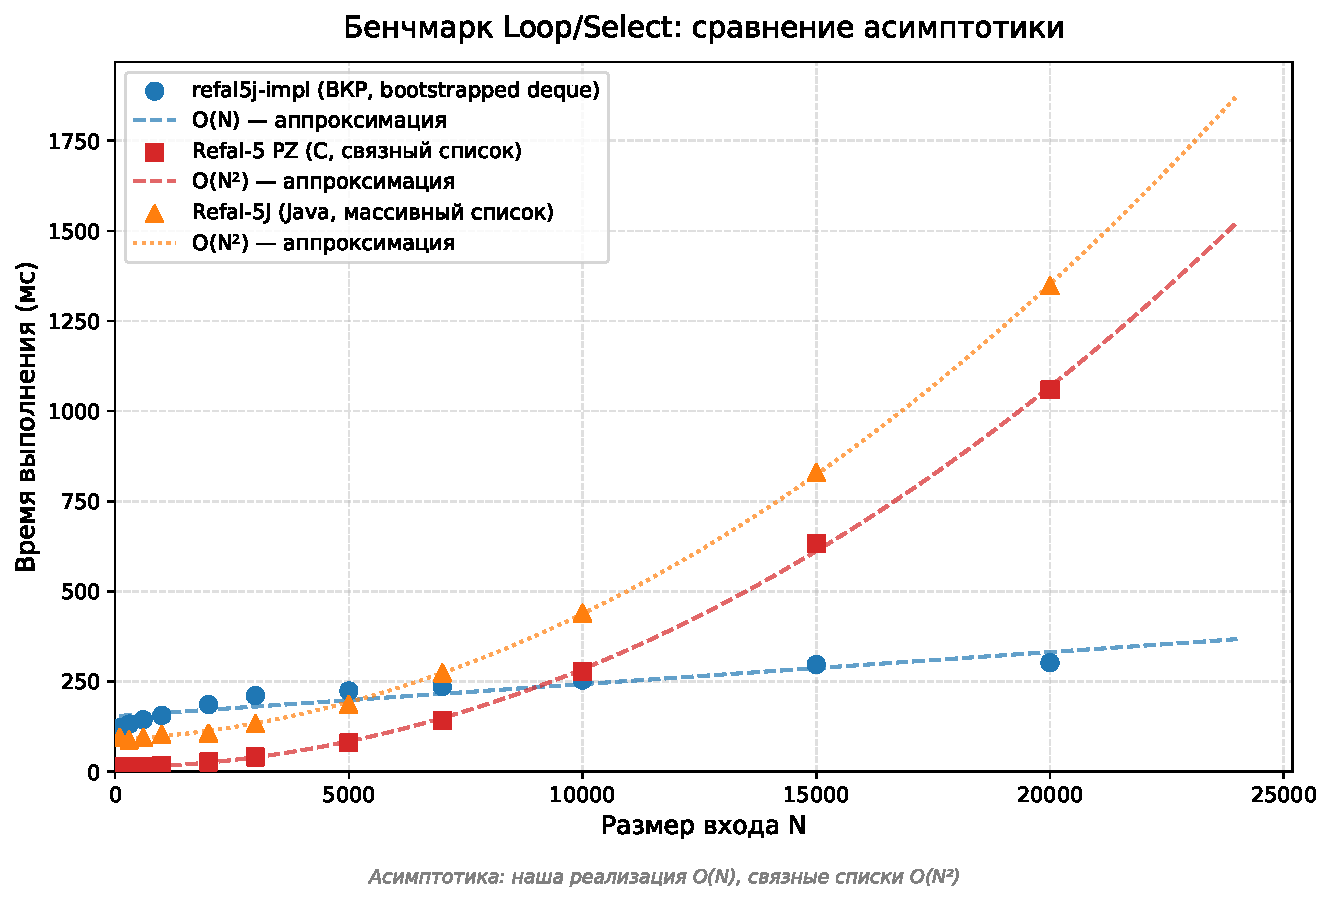
\includegraphics[width=0.95\textwidth]{loop-select-graph.pdf}
  \caption{Зависимость времени выполнения Loop/Select от размера входа N}
  \label{fig:bench-graph}
\end{figure}

\subsubsection{Обсуждение результатов}

На малых $N$ наша реализация проигрывает обоим конкурентам.
Причина простая: запуск JVM и прогрев JIT-компилятора стабильно стоят
около 120~мс, и эта плата не зависит от размера входа. Refal-5~PZ~---
нативный бинарник, его старт укладывается в единицы миллисекунд;
Refal-5J работает на той же JVM, что и мы, но тратит на инициализацию
порядка 85--90~мс.

При $N \approx 7000$ кривая Refal-5J уже догоняет нашу, при $N \approx 9000$
её перешагивает Refal-5~PZ. После этой точки квадратичный рост
конкурентов берёт своё: на $N = 10\,000$ PZ уже медленнее (277~мс против
254~мс), а на $N = 20\,000$ разрыв с PZ становится 3,5-кратным
(1059~мс против 302~мс) и 4,5-кратным с Refal-5J
(1348~мс против 302~мс).

Объяснение различия лежит в способе хранения объектного выражения.
Refal-5~PZ и Refal-5J держат выражение в виде двусвязного списка
термов: при построении нового скобочного терма \prog{(e.Acc A/B)}
на $k$-й итерации нужно скопировать всю накопленную часть длиной $k$.
$N$ итераций по $O(k)$ дают $O(N^2)$. Наш интерпретатор устроен иначе:
значение переменной идёт на стек одним объектом \prog{BulkPassive},
а сборка аргументов вызова использует \prog{Expr.concat}~--- по схеме
Окасаки это амортизированная константа независимо от длины операндов.
$N$ итераций по $O(1)$ дают $O(N)$~--- ровно то, что показывает прямая
на графике.

Стоит честно оговорить границы применимости этого замера.
Во-первых, мы измеряем время жизни всего процесса, поэтому в наши
$\approx 120$~мс на $N = 100$ входит почти исключительно запуск JVM,
а не работа интерпретатора. Во-вторых, диапазон $N$ до 20\,000 показывает
только начальный участок параболы конкурентов; на больших $N$ разрыв
будет расти быстрее, но прогон при $N \sim 10^5$ упирается в наш
тайм-аут 120~с. В-третьих, мы сравниваем интерпретатор с интерпретатором
(не с компиляторами Refal-5~PZ и Refal-5J в нативный код), чтобы
сопоставление имело смысл.


\anonsection{ЗАКЛЮЧЕНИЕ}

В ходе практики реализовано базисное подмножество Рефала-5 на Java~25.
Объектное выражение представлено иммутабельной раскрученной двусторонней
очередью \prog{Expr<T>} с двумя реализациями \prog{ShallowDeque} и
\prog{DeepDeque}; цикл нормализации построен итеративно на двух стеках
и не зависит от глубины рекурсии исходной программы. Отдельно
реализована оптимизация \prog{BulkPassive}: значение переменной попадает
на стек одной операцией, без поэлементного копирования, что превращает
типовой шаг с конкатенацией e-переменной из $O(k)$ в $O(1)$
амортизированно.

Тестовый каркас включает 143~JUnit-теста на компоненты и 79~внешних
программ, унаследованных от существующих реализаций Рефала
(\prog{refal-5j} и \prog{refal-5-framework}). По обязательной части
наборов проходит 5/5 автотестов и 18/18 десахаренных тестов;
оставшиеся отказы вызваны либо расширенным синтаксисом Рефала-5
(условия, блоки, уточнение типа через двоеточие), либо
нереализованными в базисном подмножестве встроенными функциями
(\prog{Time}, \prog{SizeOf}, \prog{Random}, \prog{GetEnv} и др.).

Сравнительный замер на программе Loop/Select подтвердил ожидание:
у нашей реализации время линейно по $N$, у Refal-5~PZ и Refal-5J
квадратично. На $N = 20\,000$ наша реализация работает в 3,5~раза
быстрее Refal-5~PZ и в 4,5~раза быстрее Refal-5J~--- несмотря на
накладные расходы запуска JVM, которые проигрывают единичным
миллисекундам нативного бинарника PZ на малых входах.

Дальнейшее развитие реализации укладывается в две линии. Первая~---
расширить набор встроенных функций до полного интерфейса Рефала-5,
чтобы покрыть оставшиеся десахаренные тесты (файловый ввод/вывод,
\prog{Time}, \prog{SizeOf}, \prog{Random}, системные функции).
Вторая~--- добавить поддержку расширенного синтаксиса Рефала-5
(условия, блоки, уточнение типа), что позволит обходиться без
внешнего рассахаривателя и запускать автотесты в их исходном виде.

\clearpage
\printbibliography[heading=bibintoc,title={СПИСОК ИСПОЛЬЗОВАННЫХ ИСТОЧНИКОВ}]

% Приложения
\clearpage
\appendix
\renewcommand{\thesection}{\Asbuk{section}}
\setcounter{section}{0}
% В приложении все \subsubsection* — без номера.
% \titleformat* меняет только шрифт, но оставляет before-code (где лежит \thesubsubsection).
% Нужно переопределить формат целиком, убрав счётчик из before-code:
\titleformat{\subsubsection}[block]{\normalfont\large\bfseries\raggedright}{}{0em}{#1}

\section{Исходный код бенчмарка Loop/Select}
\label{app:bench-src}

\lstset{language=Refal}
\begin{lstlisting}[
    caption={Бенчмарк Loop/Select (bench/loop-select.ref)},
    label={lst:loop-select-src}]
* Loop/Select benchmark - demonstrates O(N) for bootstrapped deque
* Run: java -jar target/refal5q.jar bench/loop-select.ref 10000

$ENTRY Go {
  = <TimeElapsed 0>
    <Loop Left () <Numb <Arg 1>>>
    <Prout <TimeElapsed>>;
}

Loop {
  s.Side (e.Acc) 0 = /* done */;
  s.Side (e.Acc) s.Rest
    = <Loop <Select s.Side (e.Acc A) (e.Acc B)> <- s.Rest 1>>;
}

Select {
  Left  t.Left t.Right = Right t.Left;
  Right t.Left t.Right = Left  t.Right;
}
\end{lstlisting}

\section{Инструкция по воспроизведению измерений}
\label{app:repro}

\subsubsection*{Предварительные требования}

\begin{itemize}
  \item Java~25~LTS и Apache~Maven~3.9.x (должны быть доступны в PATH);
  \item PowerShell~5.1 или новее;
  \item для сравнения с Refal-5~PZ: дистрибутив Refal-5~PZ с исполняемыми
        \prog{refc.exe} и \prog{refgo.exe};
  \item для сравнения с Refal-5J: собранный \prog{r5jc.jar} и \prog{r5jrt.jar}.
\end{itemize}

\subsubsection*{Сборка интерпретатора}

\begin{longlisting}
\caption{Сборка и запуск бенчмарка}\label{lst:repro-build}
\begin{minted}{bash}
cd refal5j-impl
mvn package -DskipTests

# our implementation only:
powershell -File bench\loop-select-bench.ps1

# with Refal-5 PZ:
powershell -File bench\loop-select-bench.ps1 -WithPZ

# with all three:
powershell -File bench\loop-select-bench.ps1 -WithPZ -WithR5J
\end{minted}
\end{longlisting}

Результаты сохраняются в \prog{bench/loop-select-results.csv}.

\subsubsection*{Построение графика}

\begin{longlisting}
\caption{Построение графика}\label{lst:repro-plot}
\begin{minted}{bash}
pip install matplotlib numpy
python bench\plot-benchmark.py --out bench\loop-select-graph.pdf
\end{minted}
\end{longlisting}

\subsubsection*{Настройка путей}

Пути к исполняемым файлам Refal-5~PZ и Refal-5J задаются переменными
\prog{\$Refal5}, \prog{\$R5JBin} и \prog{\$R5JLib} в начале файла
\prog{bench/loop-select-bench.ps1}.

\section{Реализация функций конкатенации}
\label{app:concat-impl}

Четыре вспомогательных метода класса \prog{ExprOps}, на которые
опирается \prog{Expr.concat}. Каждый обрабатывает свою комбинацию
типов операндов; диспетчер показан в листинге~\ref{lst:concat-cases}
основного текста.

\begin{longlisting}
\caption{concatSS: оба операнда ShallowDeque}\label{lst:concat-ss}
\begin{minted}{java}
private static <T> Expr<T> concatSS(ShallowDeque<T> a, ShallowDeque<T> b) {
    int total = a.size() + b.size();
    if (total <= CAPACITY) {
        ShallowDeque<T> r = a;
        for (T x : iter(b)) {
            r = r.pushBackTight(x);
        }
        return r;
    }
    // total > CAPACITY: один из буферов полный или почти полный;
    // делаем новый Deep с пустой mid.
    return DeepDeque.mkDeep(a, ShallowDeque.empty(), b, total);
}
\end{minted}
\end{longlisting}

\begin{longlisting}
\caption{concatSD: ShallowDeque + DeepDeque}\label{lst:concat-sd}
\begin{minted}{java}
private static <T> Expr<T> concatSD(ShallowDeque<T> a, DeepDeque<T> b) {
    ShallowDeque<T> bf = b.front();
    int total = b.size() + a.size();
    // Сливаем 'a' слева в b.front. Если итог влезает в один Shallow,
    // он становится новым front; иначе расщепляем на два,
    // второй идёт в начало mid.
    int bfTotal = a.size() + bf.size();
    if (bfTotal <= CAPACITY) {
        ShallowDeque<T> mergedFront = ShallowDeque.empty();
        for (T x : iter(a))  mergedFront = mergedFront.pushBackTight(x);
        for (T x : iter(bf)) mergedFront = mergedFront.pushBackTight(x);
        return DeepDeque.mkDeep(mergedFront, b.mid(), b.back(), total);
    }
    // Иначе формируем плоский массив и делим примерно пополам.
    Object[] tmp = new Object[bfTotal];
    int i = 0;
    for (T x : iter(a))  tmp[i++] = x;
    for (T x : iter(bf)) tmp[i++] = x;
    int leftLen = bfTotal - CAPACITY;
    if (leftLen < ShallowDeque.MIN_FILL) leftLen = ShallowDeque.MIN_FILL;
    int rightLen = bfTotal - leftLen;
    ShallowDeque<T> head = ShallowDeque.ofArray(tmp, 0, leftLen);
    ShallowDeque<T> tail = ShallowDeque.ofArray(tmp, leftLen, rightLen);
    // head становится новым front; tail - первым бакетом mid.
    Expr<ShallowDeque<T>> newMid = b.mid().pushFront(tail);
    return DeepDeque.mkDeep(head, newMid, b.back(), total);
}
\end{minted}
\end{longlisting}

\begin{longlisting}
\caption{concatDS: DeepDeque + ShallowDeque}\label{lst:concat-ds}
\begin{minted}{java}
private static <T> Expr<T> concatDS(DeepDeque<T> a, ShallowDeque<T> b) {
    ShallowDeque<T> ab = a.back();
    int total = a.size() + b.size();
    int abTotal = ab.size() + b.size();
    if (abTotal <= CAPACITY) {
        ShallowDeque<T> mergedBack = ShallowDeque.empty();
        for (T x : iter(ab)) mergedBack = mergedBack.pushBackTight(x);
        for (T x : iter(b))  mergedBack = mergedBack.pushBackTight(x);
        return DeepDeque.mkDeep(a.front(), a.mid(), mergedBack, total);
    }
    Object[] tmp = new Object[abTotal];
    int i = 0;
    for (T x : iter(ab)) tmp[i++] = x;
    for (T x : iter(b))  tmp[i++] = x;
    int rightLen = abTotal - CAPACITY;
    if (rightLen < ShallowDeque.MIN_FILL) rightLen = ShallowDeque.MIN_FILL;
    int leftLen = abTotal - rightLen;
    ShallowDeque<T> head = ShallowDeque.ofArray(tmp, 0, leftLen);
    ShallowDeque<T> tail = ShallowDeque.ofArray(tmp, leftLen, rightLen);
    Expr<ShallowDeque<T>> newMid = a.mid().pushBack(head);
    return DeepDeque.mkDeep(a.front(), newMid, tail, total);
}
\end{minted}
\end{longlisting}

\begin{longlisting}
\caption{concatDD: два DeepDeque --- ключевой случай O(1) аморт.}\label{lst:concat-dd}
\begin{minted}{java}
private static <T> Expr<T> concatDD(DeepDeque<T> a, DeepDeque<T> b) {
    int total = a.size() + b.size();
    ShallowDeque<T> ab = a.back();
    ShallowDeque<T> bf = b.front();
    int boundary = ab.size() + bf.size();

    Expr<ShallowDeque<T>> aMidPlus = a.mid();
    if (boundary == 0) {
        // оба пограничных пусты - ничего не добавляем.
    } else if (boundary <= CAPACITY) {
        ShallowDeque<T> merged = ShallowDeque.empty();
        for (T x : iter(ab)) merged = merged.pushBackTight(x);
        for (T x : iter(bf)) merged = merged.pushBackTight(x);
        aMidPlus = aMidPlus.pushBack(merged);
    } else {
        Object[] tmp = new Object[boundary];
        int i = 0;
        for (T x : iter(ab)) tmp[i++] = x;
        for (T x : iter(bf)) tmp[i++] = x;
        int rightLen = boundary - CAPACITY;
        if (rightLen < ShallowDeque.MIN_FILL) rightLen = ShallowDeque.MIN_FILL;
        int leftLen = boundary - rightLen;
        ShallowDeque<T> m1 = ShallowDeque.ofArray(tmp, 0, leftLen);
        ShallowDeque<T> m2 = ShallowDeque.ofArray(tmp, leftLen, rightLen);
        aMidPlus = aMidPlus.pushBack(m1).pushBack(m2);
    }

    // Рекурсивное склеивание middle-очередей: O(1) аморт. по Окасаки.
    Expr<ShallowDeque<T>> newMid = concat(aMidPlus, b.mid());
    return DeepDeque.mkDeep(a.front(), newMid, b.back(), total);
}
\end{minted}
\end{longlisting}


\end{document}